%BEGIN: Service in Smart Homes
\section{Services inside the Smart Home}\label{sec:services_in_smart_homes}
\emph{Services inside the Smart Home: A Simulation and Visualization tool.}\\

In this work \cite{lazovik2009services} the aim was to reduce the testing costs of smart homes. The goal was achieved by implementing a simulation and visualization tool which replaces services in a smart home with virtual stubs behaving just like the real hardware installed in a house. The resulting simulation tool is called ViSi.\\

The simulation scenarios were built using Google SketchUp\footnote{\url{http://www.sketchup.com}}. This was enhanced with a set of tools extending its visual representation of a house with virtual home interactive web services supporting SOAP messages. Further, the visualization component was written as a set of plug-ins for Google SketchUp.\\

\begin{figure}[H]
	\centering
	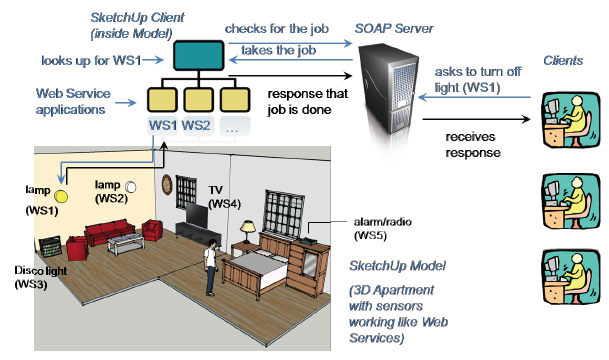
\includegraphics[width=\linewidth]{gfx/Chapter2/services_in_smarthomes}
	\caption{Architecture of the domotics simulation environment ViSi.}
	\label{fig:diasim_architecture}
\end{figure}

The simulation and visualization tool allows to simulate any possible home automation scenario, with the possibility of modelling the user and its interactions with the home.
%END: Service in Smart Homes